PROPOSITION 1.
{\em
For a community $c\in C$, if $D_c\leq M-1$ then addition of an edge within $c$ will increase its modularity.}

\begin{proof}
Recall the formulation of modularity as:
\begin{equation}\label{modularity}\small
Q(G(V,E),C)=\sum_{c\in C} (\frac{m_c}{M} - \frac{D_c^2}{4M^2})
\end{equation}
where $C$ is the community structure of $G$, $m_c$ is the total number of edges inside $c$, $D_c$ is the sum of degree of all the nodes inside a community $c\in C$, and $M=|E|$ is the total number of edges $G$.


From Equation \ref{modularity}, we see the contribution of individual community $c\in C$ in modularity as: $Q_c=\frac{m_c}{M} - \frac{D_c^2}{4M^2}$. 
where $m_c$ is the number of edges inside $c$, $M$ is the total number of edges in the graph, and $D_c$ is the sum of degrees of all the nodes in $c$. 

Addition of a new edge within $c$, the $c$'s contribution of modularity becomes:
\[
Q'_c=\frac{m_c+1}{M+1} - \frac{(D_c+2)^2}{4(M+1)^2}
\]

So the increase in modularity is $\Delta Q_c=Q'_c-Q_c$,
\[\small
\begin{split}
\Delta Q_c=&\frac{4M^2-4m_cM^2-4D_cM^2-4m_cM+2D_c^2M+D_c^2}{4(M+1)^2M^2}\\
&\geq \frac{4M^2-6D_cM^2-2D_cM+2D_c^2M+D_c^2}{4(M+1)^2M^2}\\
&\geq\frac{(2M^2-2D_cM-D_c)(2M-D_c)}{4(M+1)^2M^2}\\
&\geq 0
\end{split}
\]
The equality holds if $D_c\leq M-1$. This thus implies $(2M^2-2D_cM-D_c)\geq 0$. This proves the proposition.
\end{proof}

PROPOSITION 2.
{\em For a community $c\in C$, addition of any intra-community edge into $c$ should not split it into smaller communities.}


\begin{proof}
We will prove this proposition by contradiction.
Assume that once a new intra-community edge is added into $c$, it gets split into $k$ small modules, namely $X_1$, $X_2$, $\cdot$,$X_k$. Let $D_{X_i}$ and $e_{ij}$ be the total degree of nodes inside $X_i$ and number of edges connecting $X_i$ and $X_j$ respectively. 


Recall that the contribution of $X_i$ in the modularity value is $Q_{X_i}=\frac{m_{X_i}}{M} - \frac{D_{X_i}^2}{4M^2}$.  Before adding the edge, we have $Q_c \geq \sum_{i=1}^k Q_{X_i}$ (where $Q_c$ is the total modularity of community $c$), because otherwise all $X_i$s can be split earlier, which is not in this case. This implies that:
\[
\frac{m_c}{M}- \frac{D_c^2}{4M^2} > \sum_{i=1}^k (\frac{m_{X_i}}{M} - \frac{D_{X_i}^2}{4M^2})
\]
Since $X_1,X_2,\cdot,X_k$ are all disjoint modules of $c$, $D_c=\sum_{i=1}^k D_{X_i}$ and $m_c=\sum_{i=1}^k m_{X_i} + \sum_{i<j} e_{ij}$. This further implies that:
\[
\frac{m_c}{M}-\sum_{i=1}^k \frac{m_{X_i}}{M} > \frac{D_c^2}{4M^2}- \sum_{i=1}^k \frac{D_{X_i}^2}{4M^2}
\]
or,
\[
\sum_{i<j} e_{ij} > \frac{\sum_{i<j} D_{X_i}D_{X_j}}{2M}
\]
 
 Without loss of generality, let us assume that the new edge is added inside $X_1$. 
Since we assume that after adding the new edge into $c$, it gets split into $k$ small modules, the modularity value should increase because of the split. Therefore, the new modularity $Q'_c<\sum_{i=1}^k Q_{X_i}$. This implies that
\[\small
\begin{split}\small
& Q'_c < \sum_{i=1}^k Q_{X_i}\\
& \Leftrightarrow \frac{\sum_{i=1}^k m_{X_i} + \sum_{i<j} e_{ij} + 1}{M+1} - \frac{(\sum_{i=1}^k D_{X_i +2})^2}{4(M+1)^2}\\
& <  \frac{m_{X_1}+1}{M+1} - \frac{(D_{X_1}+2)^2}{4(M+1)^2}  + \sum_{i=2}^k  (\frac{m_{X_i}}{M+1} - \frac{D_{X_i}^2}{4(M+1)^2} )\\
&\Leftrightarrow \frac{\sum_{i=1}^k m_{X_i} + \sum_{i<j} e_{ij} + 1}{M+1} - \frac{(\sum_{i=1}^k D_{X_i +2})^2}{4(M+1)^2}\\
& < \frac{\sum_{i=1}^k m_{X_i}+1}{M+1} - \frac{(D_{X_1}+2)^2}{4(M+1)^2} - \sum_{i=2}^k \frac{D_{X_i}^2}{4(M+1)^2}\\
&\Leftrightarrow \sum_{i<i} e_{ij} < \frac{\sum_{i=1}^k D_{X_i} - 2 D_{X_1} + \sum_{i<j} D_{X_i}D_{X_j}}{2(M+1)}
\end{split}
\]
Since $\sum_{i=1}^k D_{X_i} - 2D_{X_1} < 2M$, this implies that 
\[\small
\begin{split}
\frac{\sum_{i<j}D_{X_i}D_{X_j}}{2M}  < \sum_{i<j}e_{ij} 
&< \frac{\sum_{i=1}^k D_{X_i} - 2D_{X_1} + \sum_{i\neq j}{D_{X_i}D_{X_j}}}{2(M+1)}\\
& <\frac{\sum_{i<j}D_{X_i}D_{X_j}}{2M}+1
\end{split}
\]
Therefore, the proposition holds.
\end{proof}





PROPOSITION 3.
{\em If a new edge $(u,v)$ connecting two communities $C(u)$ and $C(v)$ is introduced, $C(u)$ $($or $C(v))$ is the best candidate for $v$ (or $u$) if it should ever change its community membership.}

\begin{proof}
The method is inspired by \cite{PhysRevE.78.046115} that a vertex $u$ is influenced by two factors: $F^c_{in}(u)$ the force that keeps $u$ stay in its own community $c$, and $F^c_{out}(u)$, the force that a community $S$ imposes to $u$ in order to bring $u$ to $S$ as follows:
\[
F^c_{in}(u)=e_c^u-\frac{d_u(D_c-d_u)}{2M}
\]
and 
\[
F^S_{out}(u)=max_{S\in NC(u)} \{e_S^u - \frac{d_u D_{outS}}{2M}\}
\]
where $NC(u)$ is the set of neighboring communities of $u$, and $D_{outS}$ is the total degree of vertices outside $S$.

Now we will show that the presence of new edge $(u,v)$ will strengthen $F^{C(v)}_{out}(u)$ and weaken $F^S_{out}(u)$. In other words, we will show that $F^{C(v)}_{out}(u)$ increases while $F^S_{out}(u)$ decreases for all $S \in C \wedge S \notin \{C(u),C(v)\}$.
\[\small
\begin{split}
&F^{C(v)}_{out}(u)|_{new} - F^{C(v)}_{out}(u)|_{old}\\
&=(e_u^{C(v)}+1-\frac{(d_u+1)(d_{outC(v)}+1)}{2(M+1)} - (e_u^{C(v)} - \frac{d_ud_{outC(v)}}{2M})\\
&= \frac{2M+d_ud_{outC(v)}}{2(M+1)} - \frac{d_ud_{outC(v)}+d_{outD(v)}+d_u+1}{2(M+1)}\\
&\geq \frac{2M+d_ud_{outC(v)}}{2(M+1)} - \frac{d_u d_{outC(v)}+d_{outC(v)}+d_u+1}{2(M+1)}\\
&>0
\end{split}
\]
Therefore $F^{C(v)}_{out}(u)$ is strengthen when new edge $(u,v)$ is introduced. Furthermore, for any community $S\in C \wedge S\notin \{C(u),C(v)\}$
\[
\begin{split}
& F^{S}_{out}(u)|_{new} - F^{S}_{out}(u)|_{old}\\
&= (e^S_u-\frac{(d_u+1)d_{outS}}{2(M+1)}) - (e^S_u - \frac{d_ud_{outS}}{2M})\\
&= d_{outS}(\frac{d_u}{2M} - \frac{d_u+1}{2(M+1)})<0
\end{split}
\]

This implies that $F^S_{out}(u)$ is weakened when $(u,v)$ is added. Therefore,  the proposition holds.
\end{proof}


PROPOSITION 4.
{\em If a new edge $(u,v)$ is added into the network, then joining $u$ to $v$'s $C(v)$ community will increase the modularity value  if $\Delta Q(u,C(u),C(v)) \equiv 4(M+1)(e_{C(v)}^u+1-e_{C(u)}^u)+e_{C(v)}^u(2D_{C(v)}-2d_u-e_{C(u)}^u) - 2(d_u+1)(d_u+1+d_{C(v)}-d_{C(u)})>0$.}

\begin{proof}
Vertex $u$ will leave its current community $C(u)$ and join $v$'s community $C(v)$ if\\
\[\scriptsize
\begin{split}
& Q_{C(v)+u} + Q_{C(u)-u} > Q_{c(u)} + Q_{C(v)}\\
&\Leftrightarrow \frac{m_{C(v)}+e_{C(v)}+1}{M+1} - \frac{(d_{C(v)}+d_u+2)^2}{4(M+1)^2}+\\
&\frac{m_{C(u)} - e_{C(u)}}{M+1} - \frac{(d_{C(u)}-d_u-e_{C(u)})}{4(M+1)^2} \\
& > \frac{m_{C(v)}}{M+1} - \frac{(d_{C(v)}+d_u+2)^2}{4(M+1)^2} + \frac{m_{C(u)}}{M+1} - \frac{(d_{C(u)}+1)^2}{4(M+1)^2}\\
&\Leftrightarrow 4(M+1)(e_{C(v)} +1 -e_{C(u)}) + e_{C(u)}(2d_{C(v)} - 2d_{C(u)}-e_{C(u)})\\
& - 2(d_{C(u)}+1)(d_{C(u)}+1+d_{C(v)}-d_{C(u)})>0
\end{split}\]
\end{proof}







\begin{table*}[!t]
\centering
\caption{\label{g_metric_alg}Purity (PU), NMI and ARI values between the ground-truth and community structure obtained from individual sampling algorithms for all datasets.}
\scalebox{0.7}{
\begin{tabular}{l |>{\columncolor[gray]{0.8}} c>{\columncolor[gray]{0.8}}  c>{\columncolor[gray]{0.8}}  c|  c  c  c| ccc|ccc|ccc|>{\columncolor[gray]{0.8}}c>{\columncolor[gray]{0.8}}c>{\columncolor[gray]{0.8}}c}
\hline
\multirow{2}{*}{{\bf Dataset}} & \multicolumn{3}{c|}{{\bf \compas}} & \multicolumn{3}{c|}{{\bf SN}} & \multicolumn{3}{c|}{{\bf SE}} & \multicolumn{3}{c|}{{\bf SBFS}} & \multicolumn{3}{c|}{{\bf PIES}} & \multicolumn{3}{c}{{\bf GA}} \\\cline{2-19}
   & \multicolumn{1}{c}{PU} & \multicolumn{1}{c}{NMI} & \multicolumn{1}{c|}{ARI} & PU & NMI & ARI &PU & NMI & ARI &PU & NMI & ARI &PU & NMI & ARI & \multicolumn{1}{c}{PU} & \multicolumn{1}{c}{NMI} & \multicolumn{1}{c}{ARI} \\\hline
Facebook	  & 0.71 & 0.52 & 0.47	 & 0.43&0.34&0.26  & 0.39&0.28&0.12  &  0.53&0.41&0.18  & 0.57&0.48&0.36  & 0.76&0.61&0.52 \\
hep-th		  &	0.69&0.51&0.38 & 0.39&0.32&0.19 & 0.29&0.21&0.12 & 0.42&0.36&0.25  & 0.48&0.39&0.31 & 0.74&0.68&0.57\\
youtube		      & 0.83&0.72&0.67	 &  0.52&0.49&0.36 & 0.48&0.33&0.28  &  0.63&0.58&0.47 & 0.56&0.51&0.41  & 0.86&0.77&0.71 \\
Dblp		  &	0.72&0.65&0.58 & 0.32&0.28&0.21  & 0.29&0.21&0.16  & 0.66&0.57&0.32  & 0.48&0.39&0.31  & 0.79&0.69&0.52 \\
LFR		  & 0.76&0.69&0.55	 & 0.35&0.29&0.21  & 0.56&0.32&0.29  & 0.49&0.38&0.26  & 0.42&0.31&0.28  &  0.81&0.72&0.67 \\\hline
Average & 0.74 & 0.61 & 0.53 & 0.40 & 0.34 & 0.24 & 0.40 & 0.27 &0.19 & 0.54 & 0.46 & 0.29 & 0.50 & 0.41 & 0.33 & 0.79 & 0.69 & 0.59   \\
\hline
\end{tabular}}
\vspace{-5mm}
\end{table*}


\begin{figure}
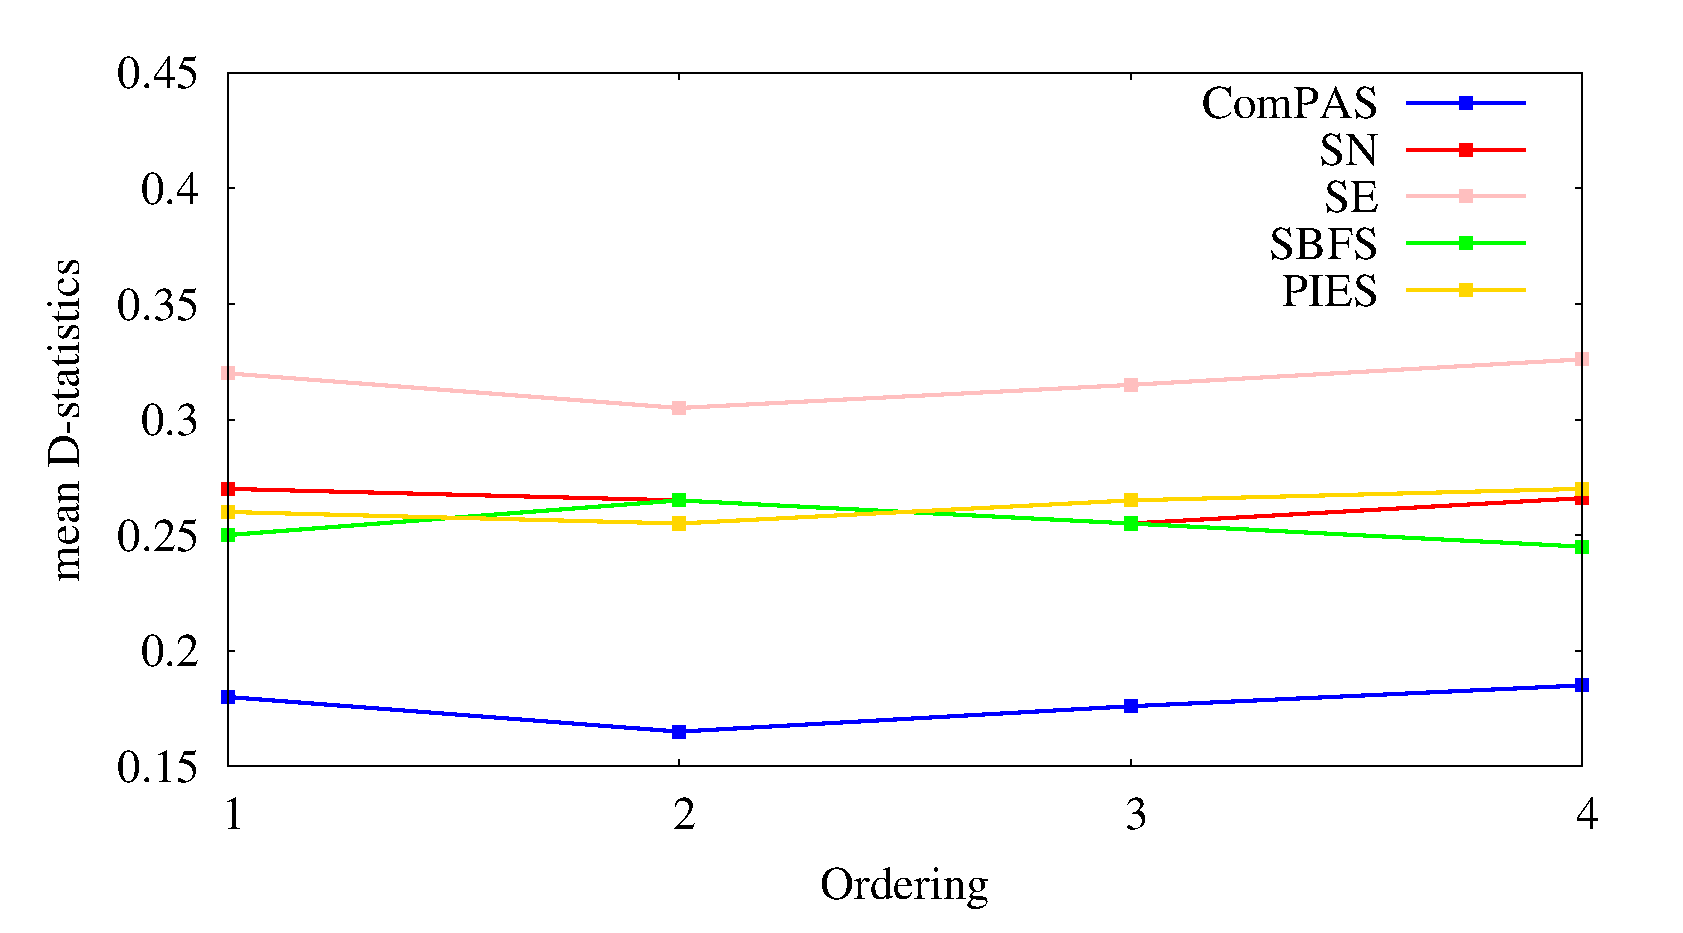
\includegraphics[scale=0.3]{figures/param_edge_order_LFR.eps}
\caption{Average D-statistics across all the topological measures for different edge ordering for LFR graph. The orderings were obtained by randomly swapping consider a pair of edges and swap their time. We do it for 20\% of the edges.}
\end{figure}

